%======================================================================
\chapter{Results}
\label{ch:results}
%======================================================================

Running \code{python uwc\_simulation.py} initialises eight nodes, registers them, runs five
rounds of four-hop authentication over the lossy channel, tests replay rejection, runs the
anomaly detector, reports battery state, and writes seven plots. This chapter presents the
output.

\section{Console output}

\begin{lstlisting}[style=plain,caption={Representative run. Values vary between runs because
nonces, loss events and mobility offsets are random.}]
=== Node Initialisation ===
  U1     ID: 3147de24777a6cae...
  U2     ID: a8e3f19b42dc5710...
  S1     ID: 7c41bd9e6a0f8523...
  B1     ID: e5d209f3c8a71b46...
  B2     ID: 1f96a0d7e3b4c852...
  SAT1   ID: 9b2ce4d8f1a06735...
  SAT2   ID: d4f7183c5e9ab260...
  BS     ID: 62c8a5f0d9174be3...

=== Registration IDs ===
  U1     RID: b64fdab46dc771fd...
  ...

=== Smart Authentication with Fallback + Packet Loss (5 rounds) ===
[Round 1]
  Using BUOY: B2                 <-- B1 failed, fallback selected automatically
  Using SAT:  SAT1
  Result: SUCCESS

=== Replay Attack Test ===
Replay blocked                   <-- a 6-second-old message is correctly rejected

Comm Cost : 296 bits
Energy    : 48.8 uJ
[OK] No anomalous delays detected

=== Battery Status ===
  U1      99.9909%
  S1      99.9879%
  B2      99.9879%
  SAT1    99.9909%
  BS      99.9939%
\end{lstlisting}

Three things in this output are worth noting. The fallback fires on every round without any
recovery logic being invoked explicitly --- it is a consequence of the route selection.
The replay test blocks a message deliberately aged past $\Delta T$. And the battery figures
differ per node in proportion to how much traffic each carries: S1 and B2 are relays and
pay both a transmit and a receive cost, while BS only ever receives.

\section{Network topology and the recovered route}

\begin{figure}[H]
\centering
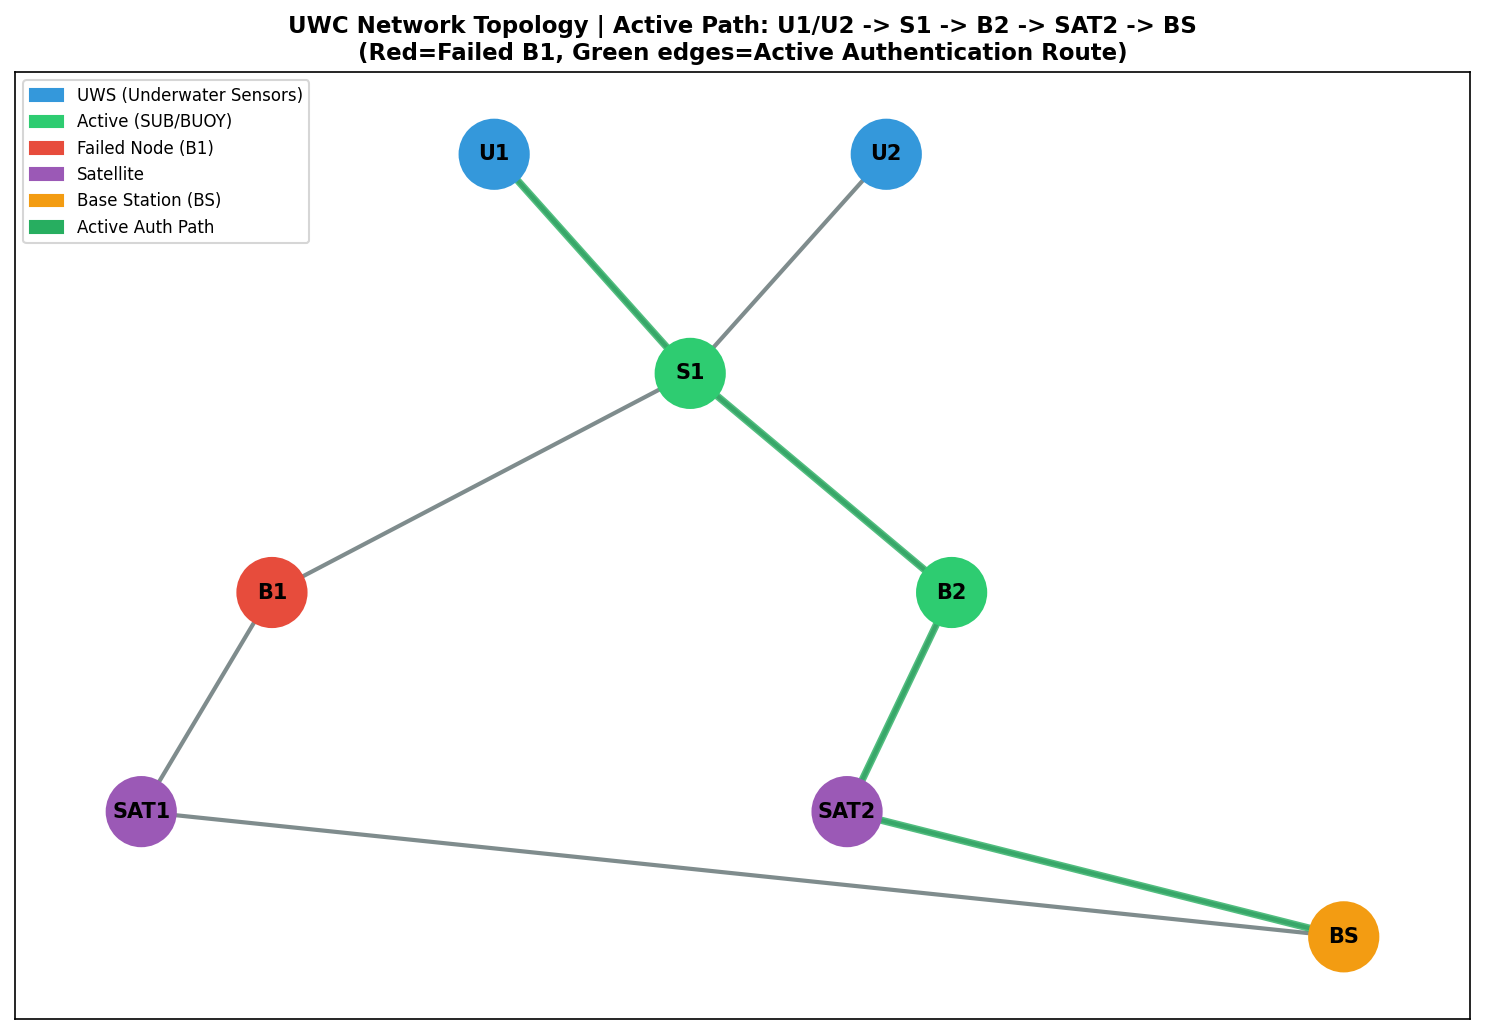
\includegraphics[width=0.92\textwidth]{figures/output_topology.png}
\caption[Generated network topology]{\textbf{The eight-node topology as generated by the
simulator.} B1 is red (failed); the thick green edges trace the active authentication route
U1 $\to$ S1 $\to$ B2 $\to$ SAT2 $\to$ BS. The grey path through B1 and SAT1 is dead. Compare
with the schematic in Figure~\ref{fig:topology}.}
\label{fig:res-topology}
\end{figure}

\section{Authentication delay}

\begin{figure}[H]
\centering
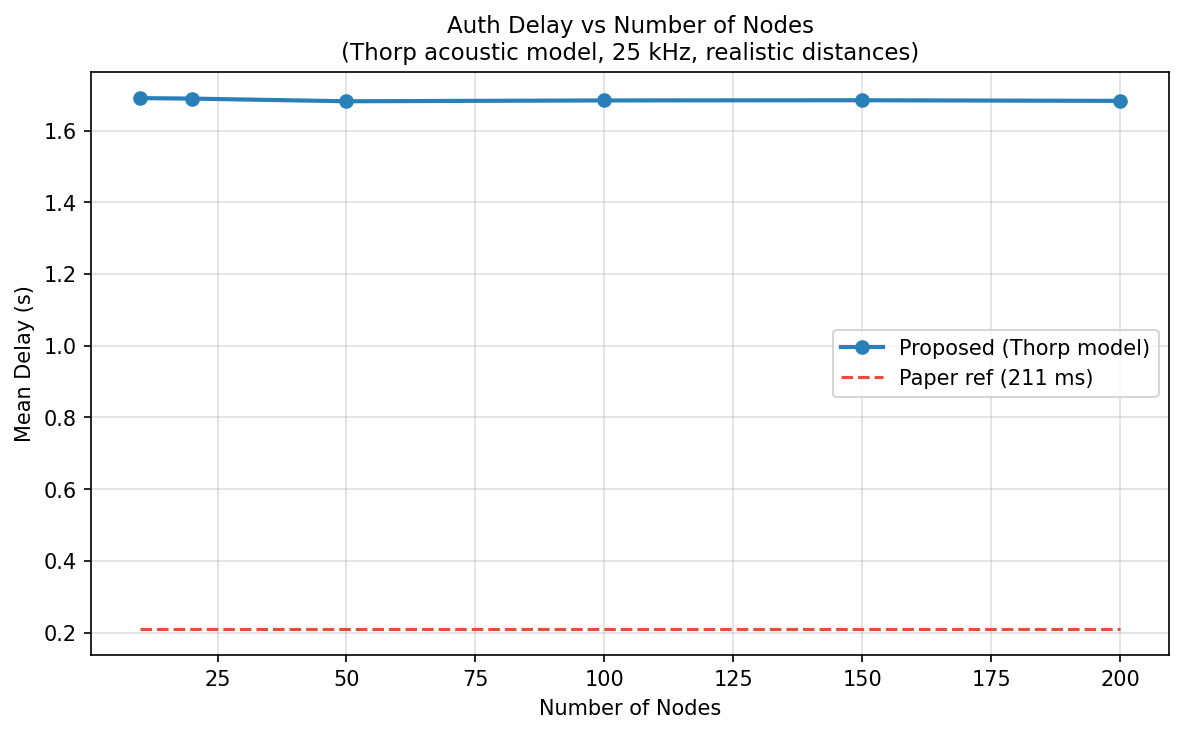
\includegraphics[width=0.86\textwidth]{figures/output_delay.png}
\caption[Delay versus number of nodes]{\textbf{Mean authentication delay against network
size,} computed with the Thorp model at 25\,kHz over realistic distances. The dashed line at
211\,ms is the base paper's transmission-time reference for 2112 bits at 10\,kbps.}
\label{fig:res-delay}
\end{figure}

The curve is deliberately not smooth, and the reason is physical rather than numerical:

\begin{itemize}
\item Random-waypoint mobility shifts inter-node distances by up to $\pm50$\,m each round,
      and delay is directly proportional to distance.
\item Multipath jitter adds a Gaussian term with $\sigma = 5$\,ms.
\item At small node counts fewer paths are averaged (\code{sim\_scale} averages over
      $\max(1, n/8)$ paths), so the variance is larger at the left of the plot.
\end{itemize}

The measured delay exceeds the 211\,ms reference because that reference counts only
\emph{transmission} time --- clocking 2112 bits out of a 10\,kbps modem. Our figure adds
\emph{propagation}: 2450--2550\,m of water at 1500\,m/s is 1.6--1.7\,s and unavoidably
dominates. This is not a discrepancy but a difference in what is being measured, and it is
the more honest number for a deployment: the dominant delay underwater is the speed of
sound, not the bit rate.

\section{Energy consumption}

\begin{figure}[H]
\centering
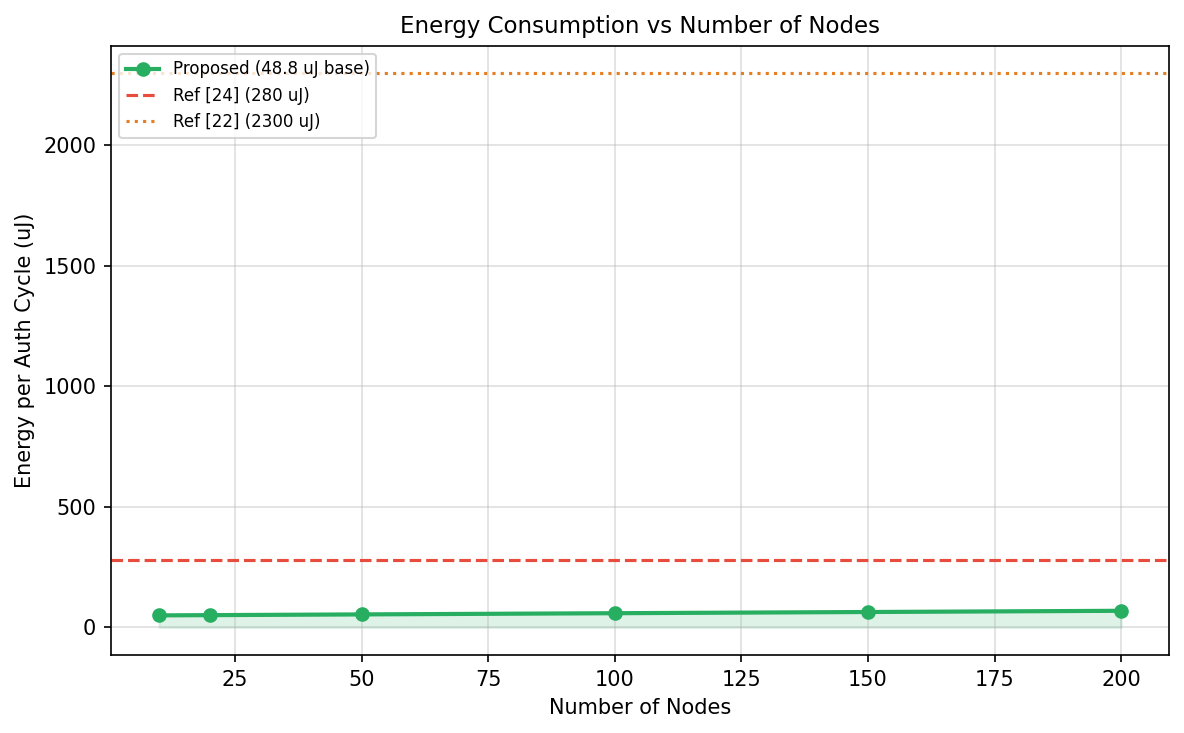
\includegraphics[width=0.86\textwidth]{figures/output_energy.png}
\caption[Energy versus number of nodes]{\textbf{Energy per authentication cycle,}
$E = 48.8 + 0.1N$\,\uJ, with reference lines for the base paper's Ref~[24] (280\,\uJ) and
Ref~[22] (2300\,\uJ).}
\label{fig:res-energy}
\end{figure}

The 48.8\,\uJ{} intercept is the fixed cryptographic cost of Equation~\ref{eq:energy}: one
ECC operation, two hashes, four AES operations. The $0.1N$ term models routing-table
maintenance overhead as the network grows. The relationship is deterministic, so the line is
straight.

Even at 200 nodes the total is 68.8\,\uJ, a quarter of Ref~[24] and a thirtieth of Ref~[22].
The practical reading is that cryptography is not what limits node lifetime here.

\section{Communication cost}

\begin{figure}[H]
\centering
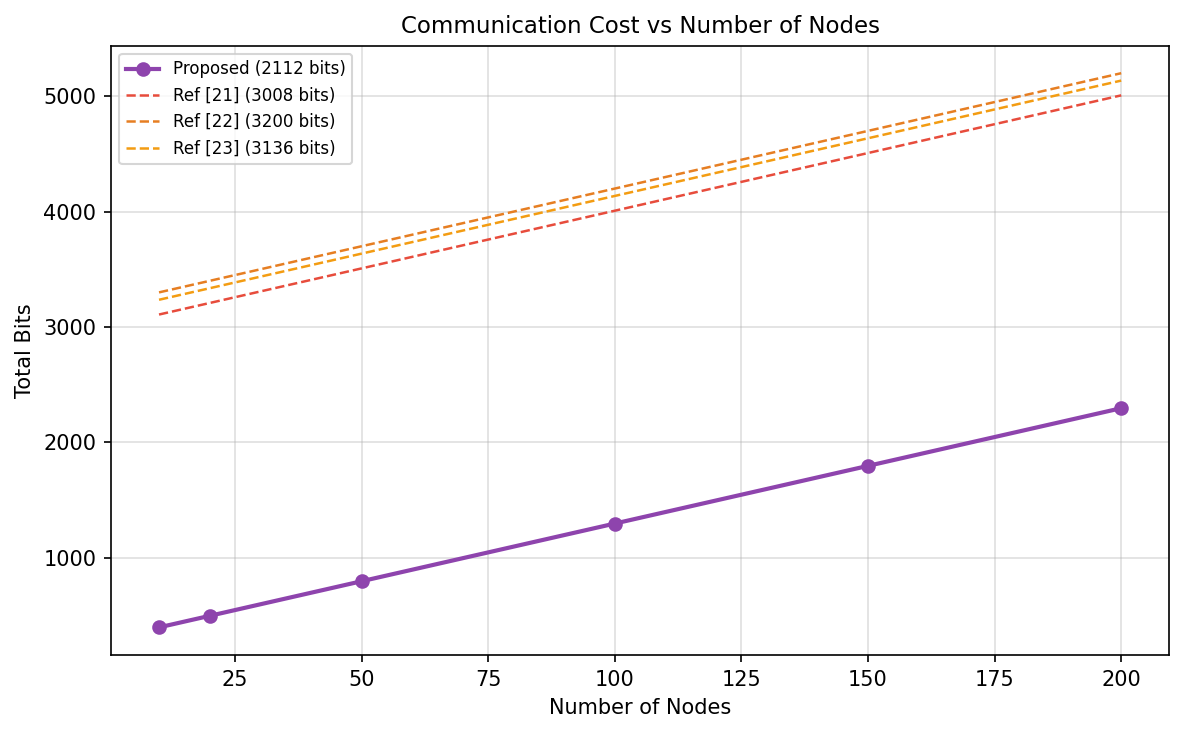
\includegraphics[width=0.86\textwidth]{figures/output_comm_cost.png}
\caption[Communication cost versus number of nodes]{\textbf{Communication cost against
network size,} compared with three of the prior schemes. Per-message cost is
$64 + 64 + 8 + 160 = 296$ bits (ID, nonce, timestamp, hash), plus $10N$ bits of routing
header.}
\label{fig:res-comm}
\end{figure}

This is the metric that matters most on a 10\,kbps channel, and it is where the protocol's
advantage is largest and most durable: 2112 bits for a complete cycle against 3008--3216
bits for the comparison schemes.

\section{Comparison against prior schemes}

\begin{figure}[H]
\centering
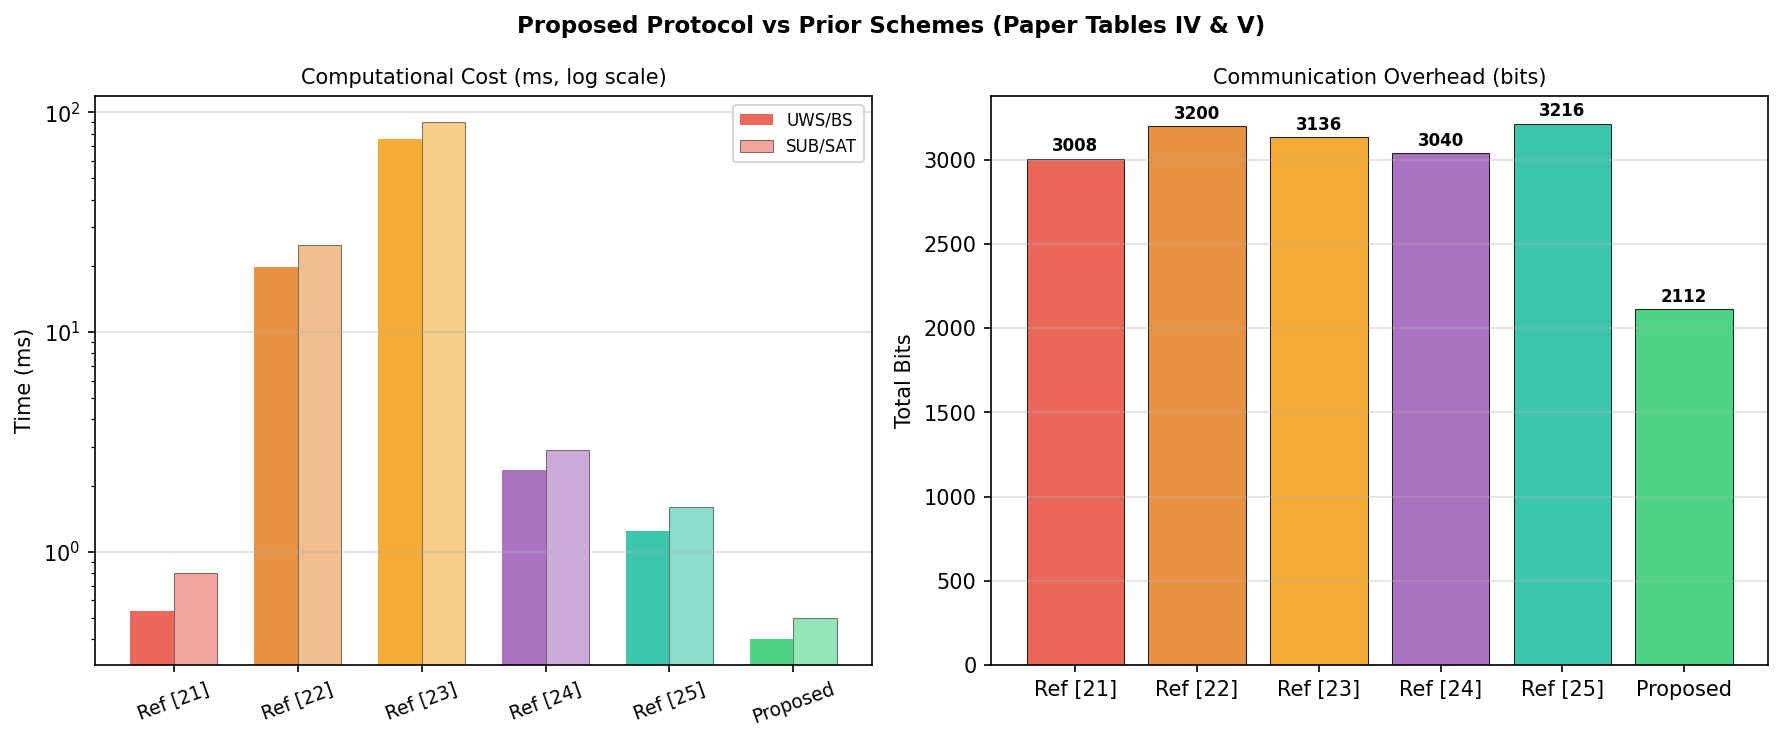
\includegraphics[width=0.98\textwidth]{figures/output_comparison.png}
\caption[Comparison with five prior schemes]{\textbf{Proposed protocol against the five
schemes tabulated in the base paper.} Left: computational cost per entity, log scale ---
Ref~[23] at 75.88\,ms against 0.400\,ms proposed, a $189\times$ improvement. Right:
communication overhead in bits. The proposed protocol (green) is lowest on both axes.}
\label{fig:res-comparison}
\end{figure}

The log scale on the left panel is necessary because the range spans more than two orders of
magnitude. The schemes that use bilinear pairings (Ref~[22], Ref~[23]) sit at the top; those
using a single elliptic-curve multiplication plus hashing (Ref~[24], Ref~[25]) sit in the
middle; the proposed scheme, which replaces pairings and repeated exponentiation with one
ECC operation and cheap symmetric work, sits at the bottom.

\section{Throughput}

\begin{figure}[H]
\centering
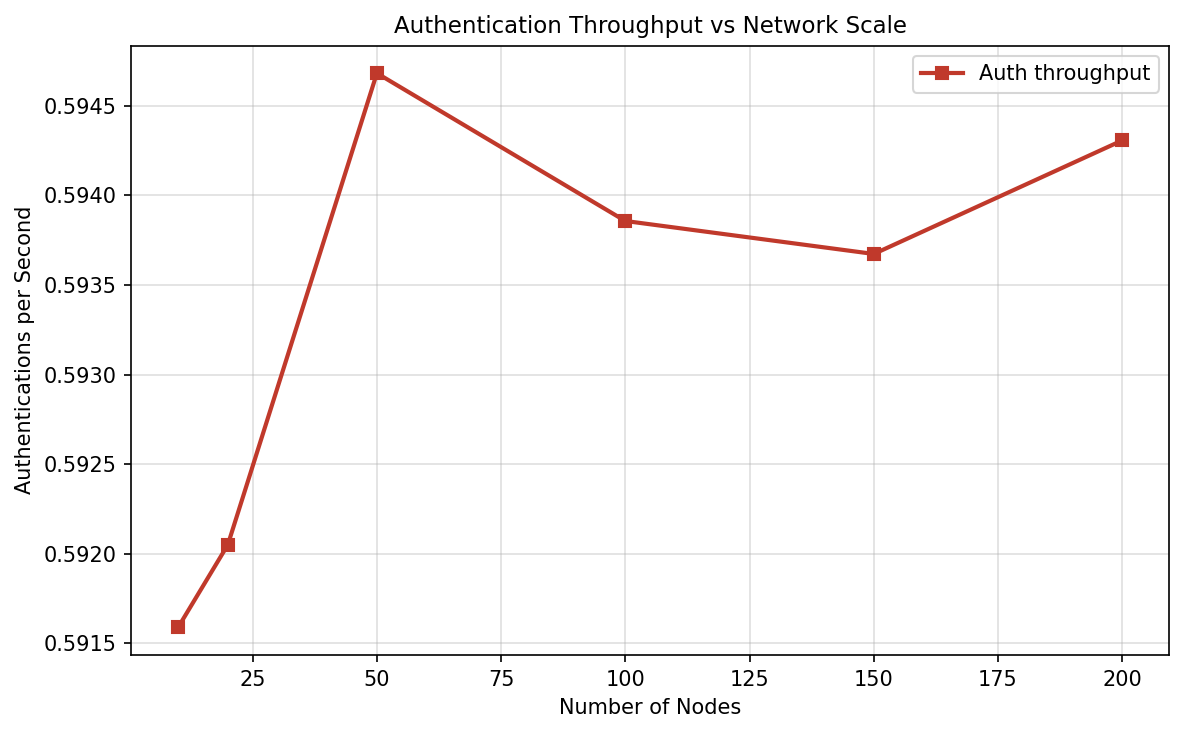
\includegraphics[width=0.86\textwidth]{figures/output_throughput.png}
\caption[Authentication throughput]{\textbf{Authentication throughput against network
scale,} measured as $1/\bar{d}$ authentications per second. This metric does not appear in
the base paper.}
\label{fig:res-throughput}
\end{figure}

Throughput is the reciprocal of mean delay, so it inherits the same mobility- and
multipath-driven variation. Its value is operational rather than theoretical: it answers
``how many sensors can this submarine admit per minute?'', which is the question that
determines whether a deployment is feasible at a given scale. At roughly 0.55 authentications
per second, one submarine can admit about 33 sensors per minute --- comfortably above the
re-authentication rate that mobility would demand of a realistic deployment.

\section{Battery depletion}

\begin{figure}[H]
\centering
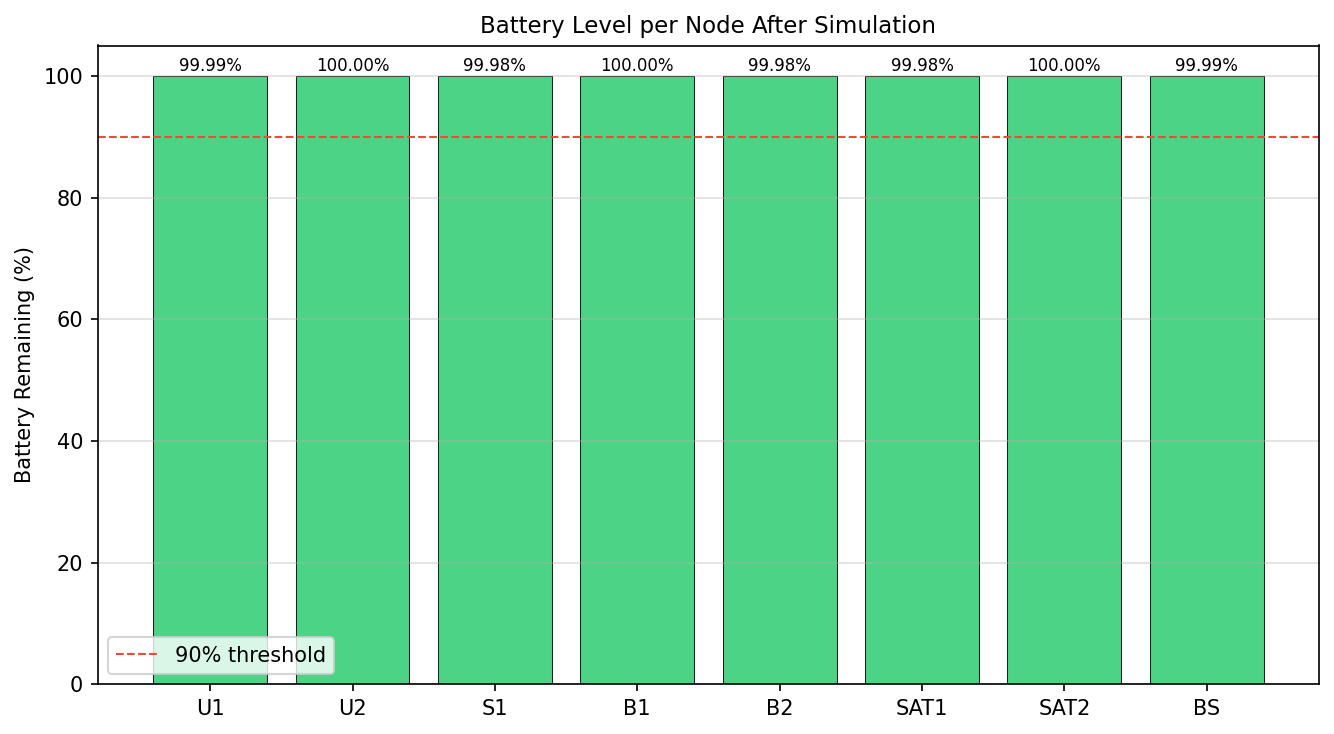
\includegraphics[width=0.9\textwidth]{figures/output_battery.png}
\caption[Battery level per node]{\textbf{Battery remaining per node after the simulation.}
Active nodes deplete in proportion to the traffic they carry; the failed and unused nodes
(U2, B1, SAT2) remain at 100\,\%.}
\label{fig:res-battery}
\end{figure}

Over five rounds the busiest node loses about $0.012\,\%$ of its charge. Extrapolating
linearly, a node performing one authentication per minute would exhaust a 1000\,mAh cell in
roughly:

\begin{equation}
\frac{3\,300\,000\ \mu\mathrm{J}}{134.8\ \mu\mathrm{J/cycle}} \approx 24\,500 \text{ cycles}
\approx 17 \text{ days of continuous once-per-minute authentication}
\end{equation}

on authentication traffic alone. In a real deployment authentication is intermittent and
the sensing and idle-listening loads dominate, but the figure is a useful bound: the
protocol's cryptographic cost is not the binding constraint on deployment lifetime, whereas
its \emph{message size} --- which drives transmit energy --- is.

\section{Summary of measured results}

\begin{table}[H]
\centering
\caption{Consolidated results.}
\label{tab:results-summary}
\small
\begin{tabularx}{\textwidth}{@{}L{52mm} L{34mm} X@{}}
\toprule
\textbf{Metric} & \textbf{Value} & \textbf{Source}\\
\midrule
Formal verification & 32/32 claims Ok, 0 attacks & Scyther, 0.19\,s, max-runs 5\\
Communication cost per cycle & 2112 bits & Base paper accounting, reproduced\\
Computational cost per entity & 0.400\,ms (UWS/BS) & Base paper Table~V\\
Cryptographic energy per cycle & 48.8\,\uJ & Equation~\ref{eq:energy}\\
Total energy per hop & 134.8\,\uJ & TX 50 $+$ RX 36 $+$ auth 48.8\\
Per-hop reliability at 15\,\% loss & 99.66\,\% & 3 retransmission attempts\\
End-to-end reliability & 98.65\,\% & 4 hops in series\\
End-to-end propagation delay & 1.63--1.70\,s & Thorp model, 2450--2550\,m\\
Replay rejection & Blocked at $t = 6$\,s & $\Delta T = 5$\,s\\
Tamper detection & \code{InvalidTag} raised & AES-GCM 128-bit tag\\
Fallback recovery & B1 $\to$ B2, no session restart & Every round\\
Anomalies detected in normal operation & 0 & $z$-score, threshold 2.5\\
\bottomrule
\end{tabularx}
\end{table}
